\chapter{Practical Implementation: MCP/A2A with FastAPI}

FastAPI, a modern, high-performance web framework for building APIs with Python, has gained significant popularity among software engineers 
due to its speed, ease of use, and robust features like automatic data validation and documentation. Its asynchronous capabilities and reliance on 
Python type hints for data validation make it particularly well-suited for implementing the server-side components of both 
Model Context Protocol (MCP) and Agent-to-Agent (A2A) protocol interactions.

\section{Setting up a FastAPI Environment for Agentic Services}
Before diving into building MCP or A2A services, a proper FastAPI development environment is essential. This typically involves:
\begin{itemize}
    \item \textbf{Python Installation:} Ensuring a compatible version of Python is installed (often Python 3.8+ for modern FastAPI features, 
    though specific MCP/A2A SDKs might have their own requirements, e.g., Python 3.10+ for some MCP tools).
    \item \textbf{Virtual Environment:} Creating an isolated Python virtual environment for the project to manage dependencies effectively.
     This can be done using \texttt{venv} or tools like \texttt{uv}.
\end{itemize}
Shell commands:
\begin{lstlisting}[language=bash]
python -m venv .venv
source .venv/bin/activate  # On Linux/macOS
# .venv\Scripts\activate    # On Windows
\end{lstlisting}

Installing FastAPI and Uvicorn: Installing the core FastAPI library and an ASGI server like Uvicorn to run the application.
Shell commands:
\begin{lstlisting}[language=bash]
pip install fastapi uvicorn
\end{lstlisting}

Alternatively, using \texttt{uv}:
Shell commands:
\begin{lstlisting}[language=bash]
uv pip install fastapi uvicorn
\end{lstlisting}

Helper Libraries for MCP/A2A: For MCP server development with FastAPI, libraries like \texttt{FastAPI-MCP} or \texttt{FastMCP} can significantly 
simplify the process by handling much of the protocol boilerplate. These would be installed similarly:
Shell commands:
\begin{lstlisting}[language=bash]
pip install fastapi-mcp  # or mcp-sdk for FastMCP related tools
\end{lstlisting}

For A2A, if a Python SDK is available (as suggested by), it would also be installed in the virtual environment. For example, \texttt{pip install a2a-sdk}.

FastAPI's native asynchronous support is a key advantage, as many interactions in agentic systems (like calling external APIs or waiting for LLM responses) 
are I/O-bound and benefit from non-blocking operations. Its use of Pydantic for data modeling ensures that incoming requests and outgoing responses conform 
to the expected schemas, which is crucial when implementing standardized protocols like MCP (JSON-RPC based) and A2A. Furthermore, FastAPI's automatic 
generation of OpenAPI documentation can be helpful for developers understanding and testing the MCP/A2A services they build.

\section{Building an MCP Server with FastAPI: A Code Walkthrough}
Let's illustrate building a simple MCP server using FastAPI. This server will expose a basic tool, for example, a function that concatenates two strings. 
We can leverage a library like \texttt{FastAPI-MCP} or \texttt{FastMCP} for this, or implement the core MCP logic if needed. For simplicity, 
we will conceptualize using a helper library that integrates with FastAPI.

\subsection*{Conceptual Example using FastAPI-MCP principles}
\texttt{FastAPI-MCP} is designed to automatically convert existing FastAPI endpoints into MCP tools or resources.
\begin{lstlisting}[language=Python]
from fastapi import FastAPI
# Hypothetical import based on library's purpose
from fastapi_mcp import FastApiMCP 
from pydantic import BaseModel

# Define the FastAPI application
app = FastAPI(title="Simple String Tools MCP Server")

# Define request model for our tool
class ConcatenateRequest(BaseModel):
    string1: str
    string2: str

# Define response model for our tool
class ConcatenateResponse(BaseModel):
    result: str

# Define a FastAPI endpoint that will become an MCP tool
@app.post("/tools/concatenate", response_model=ConcatenateResponse)
async def concatenate_strings(request: ConcatenateRequest) -> ConcatenateResponse:
    """
    Concatenates two input strings and returns the result.
    This tool is useful for joining text segments.
    """
    concatenated_string = request.string1 + request.string2
    return ConcatenateResponse(result=concatenated_string)

# Initialize and mount the FastAPI-MCP server
# The library would inspect 'app' for endpoints and expose them via MCP.
# It would use endpoint path, docstrings, and Pydantic models for MCP tool schema.
mcp_server = FastApiMCP(
    app,
    name="StringToolsServer",
    description="An MCP server providing basic string manipulation tools.",
    base_url="http://localhost:8000" # URL where this FastAPI app runs
)
mcp_server.mount() # This would typically expose an /mcp endpoint

if __name__ == "__main__":
    import uvicorn
    uvicorn.run(app, host="0.0.0.0", port=8000)
\end{lstlisting}
In this example:
We define a standard FastAPI application and an endpoint (\texttt{/tools/concatenate}). Pydantic models (\texttt{ConcatenateRequest}, 
\texttt{ConcatenateResponse}) define the input and output schemas for the tool. FastAPI uses these for validation and OpenAPI documentation, 
and \texttt{FastAPI-MCP} would leverage them to generate the MCP tool's input and output schemas. The docstring of the \texttt{concatenate\_strings} 
function would serve as the description for the MCP tool, helping the LLM understand what the tool does. \texttt{FastApiMCP(app,...).mount()} is 
the key step where the library integrates with the FastAPI app instance. It would typically scan the app's routes, identify those intended as 
MCP tools (perhaps based on decorators or conventions), and expose them via a dedicated MCP endpoint (e.g., \texttt{/mcp}). 
This endpoint would handle incoming JSON-RPC messages according to the MCP specification.

\subsection*{Conceptual Example using FastMCP principles}
FastMCP often uses decorators to explicitly define MCP tools from Python functions.
\begin{lstlisting}[language=Python]
from fastapi import FastAPI
from fastmcp import FastMCP # Hypothetical import based on library's purpose
import uvicorn

# Create an MCP server instance
mcp_logic = FastMCP("SimpleStringTools")

# Define a Python function and decorate it as an MCP tool
@mcp_logic.tool()
def concatenate(string1: str, string2: str) -> str:
    """
    Concatenates two input strings.
    Use this to join pieces of text.
    Parameters:
        string1 (str): The first string.
        string2 (str): The second string.
    Returns:
        str: The combined string.
    """
    return string1 + string2

# Create a FastAPI app to host the MCP server logic
app = FastAPI()

# Mount the FastMCP logic onto a FastAPI route (e.g., /mcp)
# This step would involve specific integration code provided by FastMCP
# to handle JSON-RPC requests at this endpoint and dispatch to mcp_logic.
# For example: app.include_router(mcp_logic.as_fastapi_router(), prefix="/mcp")

# A simplified conceptual mounting:
@app.post("/mcp")
async def handle_mcp_request(request_data: dict): # Actual handling is more complex
    # FastMCP would provide a handler here to process JSON-RPC,
    # invoke 'concatenate' if requested, and return JSON-RPC response.
    # This is a placeholder for that complex logic.
    if request_data.get("method") == "tool_concatenate": # Simplified check
        params = request_data.get("params", {})
        result = concatenate(params.get("string1"), params.get("string2"))
        return {"jsonrpc": "2.0", "result": result, "id": request_data.get("id")}
    return {"jsonrpc": "2.0", "error": {"code": -32601, "message": "Method not found"}, \
"id": request_data.get("id")}

if __name__ == "__main__":
    uvicorn.run(app, host="0.0.0.0", port=8000)
\end{lstlisting}
In this FastMCP style:
An \texttt{FastMCP} instance (\texttt{mcp\_logic}) is created. The \texttt{@mcp\_logic.tool()} decorator registers the \texttt{concatenate} 
function as an MCP tool. FastMCP would use the function signature (type hints) and docstring to generate the MCP tool schema.
 The FastMCP instance then needs to be exposed via a FastAPI endpoint (e.g., \texttt{/mcp}). 
 The library would provide mechanisms to translate incoming JSON-RPC requests at this endpoint into calls to the registered Python functions 
 and format the responses correctly.

Libraries like \texttt{FastAPI-MCP} and \texttt{FastMCP} aim to abstract away the low-level details of the MCP protocol 
(like JSON-RPC message parsing, request dispatching, and response formatting), allowing software engineers to focus on implementing 
the actual business logic of their tools. This significantly lowers the barrier to entry for creating MCP-compliant servers.

\section{Illustrative Block Diagram of the FastAPI MCP Service}
To visualize how a FastAPI application serves as an MCP server, consider the following components and their interactions:
\begin{figure}[htbp]
    \centering
    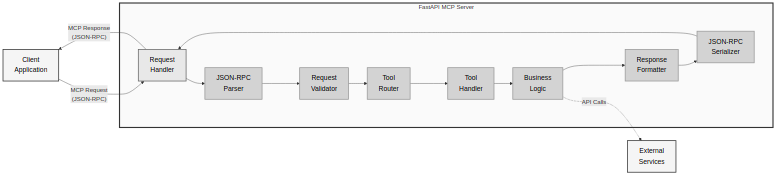
\includegraphics[width=\textwidth]{diagrams/mcp_server.png}
    \caption{Block Diagram of the FastAPI MCP Service Architecture.}
    \label{fig:mcp_server_diagram}
\end{figure}
\subsection*{Explanation of Diagram}
\begin{itemize}
    \item \textbf{MCP Client / LLM Agent Host:} This is the application (e.g., an IDE with an AI assistant, Claude Desktop, or a custom Python 
    script running an agent) that wants to use a tool. It constructs an MCP request (a JSON-RPC message).
    \item \textbf{Transport Layer:} The request is sent over a chosen transport (stdio for local servers, HTTP/SSE for remote servers) to the FastAPI application.
    \item \textbf{FastAPI Application (MCP Server):}
    \begin{itemize}
        \item \textbf{Transport Handler:} The FastAPI application (via Uvicorn or another ASGI server) listens for incoming requests on the configured transport.
        \item \textbf{MCP Protocol Layer:} A library like \texttt{FastAPI-MCP} or \texttt{FastMCP}, or custom MCP handling logic, 
        parses the incoming JSON-RPC message. It identifies that this is a request to call a specific MCP tool.
        \item \textbf{FastAPI Router:} The protocol layer dispatches the call to the appropriate FastAPI endpoint 
        (if using \texttt{FastAPI-MCP} where endpoints are tools) or to the Python function registered as an MCP tool (if using FastMCP-style decorators).
        \item \textbf{FastAPI Endpoint / Decorated Function:} This is the Python code written by the developer that implements the tool's logic.
        \item \textbf{Business Logic / API Client:} The tool's implementation might involve direct computation, calling other internal services,
         or making requests to external APIs or databases.
    \end{itemize}
    \item \textbf{Response Path:} The result from the business logic is returned to the FastAPI endpoint/function, then formatted by the 
    MCP Protocol Layer into a JSON-RPC response, and sent back to the MCP Client via the Transport Handler.
    \item \textbf{Underlying Data Source / External API:} If the MCP tool is a wrapper around an existing service, the Business 
    Logic component will interact with this external system.
\end{itemize}
This diagram illustrates the flow of an MCP tool invocation request from an agent to a FastAPI-based MCP server and back, highlighting 
the layers of abstraction provided by FastAPI and MCP helper libraries.

\section{Exposing A2A Endpoints with FastAPI (Conceptual Overview \& Block Diagram)}
FastAPI can also serve as the framework for hosting "remote agents" in an Agent-to-Agent (A2A) communication scenario. In A2A, 
one agent (the client agent) discovers and delegates tasks to another agent (the remote agent, which acts as a server).

\subsection*{Conceptual Overview}
\begin{itemize}
    \item \textbf{A2A Server (Remote Agent) with FastAPI:} A FastAPI application can expose the necessary HTTP endpoints required by the A2A protocol.
    \item \textbf{Agent Card Discovery:} The remote agent needs to make its "Agent Card" discoverable. 
    This is typically a JSON file served from a well-known path, often \texttt{/.well-known/agent.json} on the agent's domain. 
    A FastAPI route can be set up to serve this static JSON file or generate it dynamically.
    \item \textbf{Task Handling Endpoints:} The A2A protocol defines how tasks are submitted and managed. A FastAPI application would need endpoints to:
    \begin{itemize}
        \item Receive new task requests (e.g., at a \texttt{/run} endpoint as seen in some examples, or specific paths like \texttt{/tasks/send} 
        or \texttt{/message/send} as per evolving A2A specifications).
        \item Handle message exchanges related to an ongoing task.
        \item Provide status updates for long-running tasks, potentially using Server-Sent Events (SSE) for streaming responses.
    \end{itemize}
    \item \textbf{A2A Python SDK:} If a mature A2A Python SDK is available (as suggested by), it would likely provide utilities to 
    simplify the implementation of these A2A server-side functionalities within a FastAPI application, handling A2A message parsing, 
    task lifecycle management, and response formatting.
    \item \textbf{Agent Core Logic:} Behind these FastAPI endpoints, the remote agent's core logic (which might involve an LLM, 
    its own tools possibly accessed via MCP, and memory) would process the tasks delegated to it.
\end{itemize}

\subsection*{Illustrative Block Diagram of FastAPI-based A2A Communication}
\begin{figure}[htbp]
    \centering
    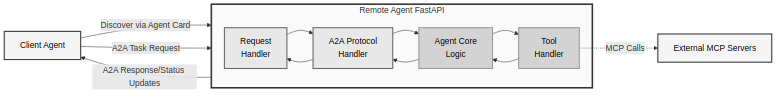
\includegraphics[width=\textwidth]{diagrams/mcp_a2a.png}
    \caption{Block Diagram of the FastAPI A2A Service Architecture.}
    \label{fig:mcp_a2a_diagram}
\end{figure}

\subsection*{Explanation of Diagram}
\begin{itemize}
    \item \textbf{Discovery:} The Client Agent (which could also be a FastAPI application or any A2A-compliant agent) first discovers
     the Remote Agent by fetching its Agent Card (a JSON file) from a well-known HTTP endpoint hosted by the Remote Agent's FastAPI application.
    \item \textbf{Task Request:} The Client Agent sends an A2A task request (a JSON-RPC message over HTTP POST) to a specific endpoint on 
    the Remote Agent's FastAPI server (e.g., \texttt{/run} or \texttt{/tasks/send}).
    \item \textbf{Remote Agent (FastAPI App 2 - A2A Server):}
    \begin{itemize}
        \item \textbf{FastAPI HTTP Endpoints:} The FastAPI app receives the request.
        \item \textbf{A2A Protocol Handler:} This layer (potentially facilitated by an A2A SDK) parses the A2A message, validates it, and 
        manages the A2A task lifecycle.
        \item \textbf{Agent Core Logic:} The task is delegated to the Remote Agent's core logic, which uses its LLM, planning capabilities, 
        and memory to process the task.
        \item \textbf{MCP Client (Optional):} The Remote Agent's core logic might itself be an MCP client, using MCP to access its 
        own specialized tools or data sources (represented by External MCP Servers).
    \end{itemize}
    \item \textbf{A2A Response/Status Updates:} The Remote Agent's A2A Protocol Handler formats the result or status updates into 
    A2A-compliant JSON-RPC messages and sends them back to the Client Agent, possibly over HTTP response or an SSE stream for long-running tasks.
\end{itemize}
This diagram illustrates how FastAPI can serve as the web framework for both the external-facing A2A protocol endpoints and for 
orchestrating the internal workings of a remote agent. A sophisticated agent might act as an MCP client to gather information or use tools, 
and simultaneously act as an A2A server to offer its specialized capabilities to a wider network of collaborating agents. 
This composability is key to building complex, multi-functional agentic systems.

